\section{Implementation}

\begin{figure}[H]
\centering
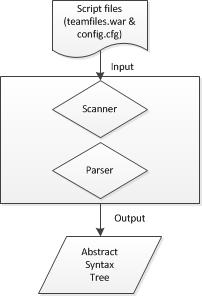
\includegraphics[scale=1]{rapport/6/figures/parser}
\label{fig:parser}
\caption{Parser}
\end{figure}

\subsubsection{Getting the data - and validating it}
Inside the simulator figure \ref{fig:simulator} we implemented a $GameDataRetriever$ class which should retrieve data from the Decorated Abstract Syntax Tree, so we have reused the visitor pattern to run through the tree and collect all the data needed to run the simulator. After all the data have been retrieved from the DAST we have to validate if the data is correct. By correct we mean that e.g. in the config.cfg file a $Maxima$ is present, and if the teamfiles.war contains larger numbers than the $Maxima$ requires, there will be an error. The config.cfg file contains standards for which the programmers teamfiles.war will be assigned to if they haven't assigned their own constants. An example: if the teamfile.war does contain a regiment with some size and a name of the regiment, but nothing more, the regiment will then be assigned the default/standard values, if the standard values is nowhere to be found in the config.cfg file there will be an error as well.

\begin{figure}[H]
\centering
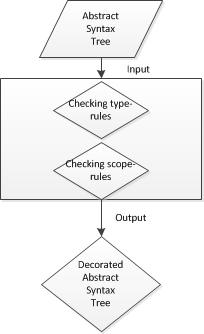
\includegraphics[scale=1]{rapport/6/figures/contextual_analyzer}
\label{fig:contextual_analyzer}
\caption{Contextual Analyzer}
\end{figure}

\begin{figure}[H]
\centering
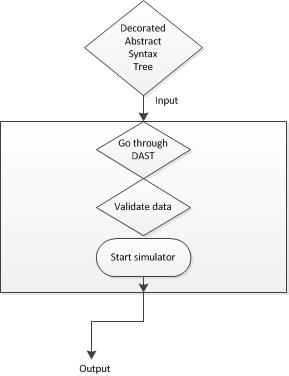
\includegraphics[scale=1]{rapport/6/figures/simulator}
\label{fig:simulator}
\caption{Simulator}
\end{figure}


\subsection{Simulation}

After getting the data and validating it, and we are sure that the simulator can run, we are now able to start the simulator with the required data. 
Starting the simulator requires some part of computation, the starting position of all the regiments, which player is allowed to start. This is here the interpreter is useful, by using an interpreter it can compute all the damage done from each regiment, and what kind of $gameState$ the simulator is in right now. The interpreter is doing all the computations by looking at the $gameStates$ present status, and reading the next input and then computing the next $gameState$ and updating the screen with the new input, and then it is the next regiments turn. This is a loop that will continue until any player on the grid will win, or the program gets terminated.


%Interpreter eksekver en behaviour





